\documentclass[conference]{IEEEtran}
\IEEEoverridecommandlockouts
% The preceding line is only needed to identify funding in the first footnote. If that is unneeded, please comment it out.
\usepackage{cite}
\usepackage{amsmath,amssymb,amsfonts}
\usepackage{algorithmic}
\usepackage{graphicx}
\usepackage{textcomp}
\usepackage{xcolor}
\def\BibTeX{{\rm B\kern-.05em{\sc i\kern-.025em b}\kern-.08em
    T\kern-.1667em\lower.7ex\hbox{E}\kern-.125emX}}

\begin{document}

\title{A Game Theory Based Collusion Aware Auction Framework for Agentic Compute Markets
\thanks{Identify applicable funding agency here. If none, delete this.}
}

\author{
\IEEEauthorblockN{1\textsuperscript{st} Om Ashok Nalage}
\IEEEauthorblockA{\textit{Department of Computer Science and Engineering} \\
\textit{Visvesvaraya National Institute of Technology (VNIT)}\\
Nagpur, India \\
omashoknalage@gmail.com}
\and
\IEEEauthorblockN{2\textsuperscript{nd} Prabhat Kumar Prince}
\IEEEauthorblockA{\textit{Department of Computer Science and Engineering} \\
\textit{Visvesvaraya National Institute of Technology (VNIT)}\\
Nagpur, India \\
email address or ORCID}
\and
\IEEEauthorblockN{3\textsuperscript{rd} Rajat Samarth}
\IEEEauthorblockA{\textit{Department of Computer Science and Engineering} \\
\textit{Visvesvaraya National Institute of Technology (VNIT)}\\
Nagpur, India \\
rsamarth22@gmail.com}
\and
\IEEEauthorblockN{4\textsuperscript{th} Sakshi Pore}
\IEEEauthorblockA{\textit{Department of Computer Science and Engineering} \\
\textit{Visvesvaraya National Institute of Technology (VNIT)}\\
Nagpur, India \\
poresakshi344@gmail.com}
}

\maketitle

\begin{abstract}
This paper studies agentic compute markets where autonomous bidders may collude. We compare a baseline second price auction to an improved design with collusion aware bid enforcement and machine learning based round level monitoring. Simulations use many agents and repeated rounds with multi trial aggregation. We report average payment and welfare, detector performance, and include comparison plots for payment and welfare versus round.
\end{abstract}

\begin{IEEEkeywords}
game theory, vickrey auction, collusion detection, agentic markets, compute marketplace, adaptive enforcement
\end{IEEEkeywords}

\section{Introduction}
Market style allocation of compute for AI workloads increasingly relies on software agents that bid on behalf of users. Coordinated bidding can depress prices and harm efficiency. This work presents a reproducible simulation that compares baseline clearing to an improved pipeline with adaptive enforcement while preserving a second price payment rule.

\section{Methodology (Summary)}
Agents draw valuations from a normalized hardware table. Each round, honest and collusive bidding modes produce a bid vector. Round level features summarize bid dispersion and temporal structure. The improved system adjusts bids before clearing using an online risk score. Outcomes record second price payment and a welfare proxy tied to the winning bid. The implementation exports figures under a graphs folder.

\section{Experimental Setup}
Default protocol uses one hundred fifty agents, two hundred rounds per trial, and twenty seeded trials. The dataset path is set in the project configuration file. Compile this paper from the project root so relative paths to PNG files resolve.

\section{Results}

\subsection{Aggregate metrics}
Table~\ref{tab:results} summarizes trial level means and standard deviations from the same pipeline that generates Fig.~\ref{fig:paycomp} and Fig.~\ref{fig:welfarecomp}. Update the numeric cells after each full run of \texttt{python main.py} if you change parameters.

\begin{table}[htbp]
\caption{Multi trial simulation summary (twenty trials, stratified detector evaluation per trial).}
\label{tab:results}
\begin{center}
\begin{tabular}{|l|c|}
\hline
\textbf{Metric} & \textbf{Value} \\
\hline
Basic mean payment & $3.8573 \pm 0.0009$ \\
Improved mean payment & $4.6247 \pm 0.0190$ \\
Basic mean welfare & $3.8711 \pm 0.0013$ \\
Improved mean welfare & $4.6399 \pm 0.0190$ \\
\hline
Payment gain (Improved vs Basic) & $19.90\%$ \\
Welfare gain (Improved vs Basic) & $19.86\%$ \\
\hline
Accuracy & $0.9200 \pm 0.0267$ \\
ROC-AUC & $0.9284 \pm 0.0291$ \\
Precision & $0.9224 \pm 0.0364$ \\
Recall & $0.9146 \pm 0.0465$ \\
FPR & $0.0773 \pm 0.0382$ \\
FNR & $0.0854 \pm 0.0465$ \\
\hline
\end{tabular}
\end{center}
\end{table}

\subsection{Comparison graphs}
Fig.~\ref{fig:paycomp} and Fig.~\ref{fig:welfarecomp} show the baseline versus improved curves in standard IEEE figure layout, with one graph per figure and consistent axis interpretation.

\begin{figure}[!t]
\centering
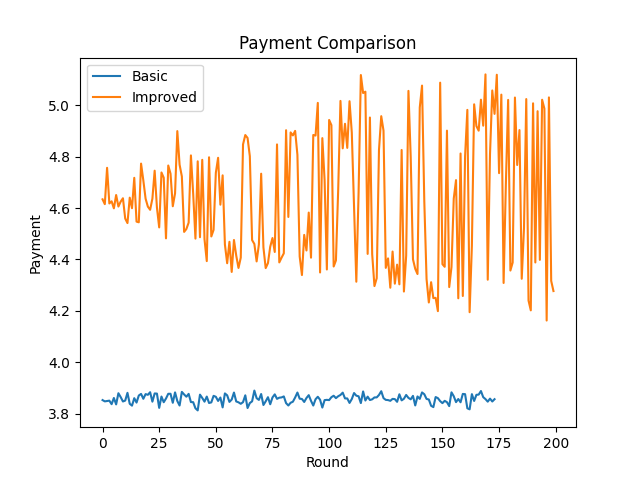
\includegraphics[width=\columnwidth]{graphs/comparison_payments.png}
\caption{Payment comparison for Basic and Improved systems (axes: Round, Payment).}
\label{fig:paycomp}
\end{figure}

\begin{figure}[!t]
\centering
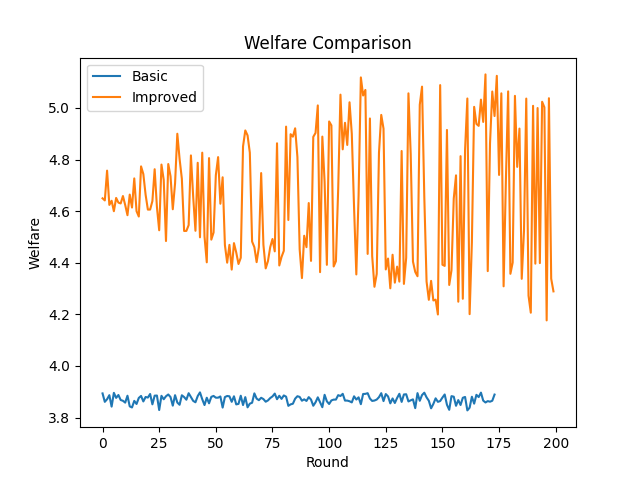
\includegraphics[width=\columnwidth]{graphs/comparison_welfare.png}
\caption{Welfare comparison for Basic and Improved systems (axes: Round, Welfare).}
\label{fig:welfarecomp}
\end{figure}

\section{Discussion}
Detector metrics in Table~\ref{tab:results} reflect a synthetic task and should not be read as guaranteed real world performance. Cross dataset tests and noisier labels are recommended before deployment claims.

\section{Conclusion}
We presented a game theory motivated collusion aware auction simulation with clear baseline versus improved comparison, quantitative aggregation in Table~\ref{tab:results}, and visual evidence in Fig.~\ref{fig:paycomp} and Fig.~\ref{fig:welfarecomp}.

\section*{Acknowledgment}
\textbf{Under the guidance of Dr. Anshul Agarwal.}

\begin{thebibliography}{00}
\bibitem{b1} W. Vickrey, ``Counterspeculation, auctions, and competitive sealed tenders,'' \emph{Journal of Finance}, vol. 16, no. 1, pp. 8--37, 1961.
\bibitem{b2} F. Pedregosa \emph{et al.}, ``Scikit-learn: Machine learning in Python,'' \emph{JMLR}, vol. 12, pp. 2825--2830, 2011.
\bibitem{b3} T. Fawcett, ``An introduction to ROC analysis,'' \emph{Pattern Recognition Letters}, vol. 27, no. 8, pp. 861--874, 2006.
\end{thebibliography}

\vspace{12pt}
\color{red}
IEEE conference templates contain guidance text for composing and formatting conference papers. Please ensure that all template text is removed from your conference paper prior to submission to the conference. Failure to remove the template text from your paper may result in your paper not being published.

\end{document}
